%\section{Motivation}
OCamlyacc generates a parser from a set rules that are defined by the user in syntax similar to BNF, and OCamllex 
translates a set of regular expressions to a lexical analyzer. The goal of gt is to allow the user to easily 
define a context-free grammar in one file and then generate the corresponding parser, lexical analyzer and syntax
trees based on the rules defined in the file. In addition, gt adds support for EBNF notation. Here is an example 
of an input file: \\
\begin{gt} 
lists

Grammar : grammar -> { olist }*.

OList : olist -> LSBRACKET [ element { SEMI element }* ] RSBRACKET.

Element :  element -> VAR | INT.

LSBRACKET = "[".
RSBRACKET = "]".
SEMI = ";".

VAR = {{ ['a'-'z''A'-'Z'] ['a'-'z''A'-'Z''0'-'9''_']* }}.
INT = {{ ['0'-'9']+ }}.
\end{gt}\ \\
Gt takes a file in the format shown above and generates multiple OCaml source files, as show in Figure 1.1. These
files can then be compiled to an executable.

\begin{figure}[h!]
  \centering
  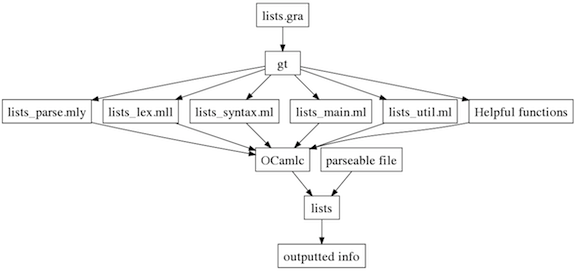
\includegraphics[width=5.3in]{./intro/gt.png}
  \caption{}
\end{figure}\ \\
After the files in Figure 1.1 are compiled the executable is ready to parse programs such as, [ 0 ; a ; 1 ], to
syntax trees like the one shown in Figure 1.2. The syntax tree in Figure 1.2 was actually generated, in Graph-viz
format, by the same executable.

Along with the ability to easily generate parsers, gt generates many useful functions. For example dump\_gviz,
which creates a Graph-Viz file containing a syntax tree definition for a given parseable file. The file names listed below are 
some of names corresponding to the gt generated files. Below the keyword \textit{grammar\_name} refers to the name of the 
grammar. For example, for the definition above \textit{grammar\_name} would would refer to lists \textit{lists}. 

\begin{figure}[h!]
  \centering
  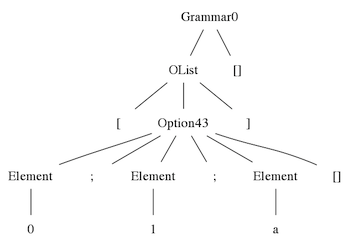
\includegraphics[width=4.5in]{./intro/lists.png}
  \caption{}
\end{figure}\ \\
\[
\begin{array}{ll}
\textnormal{\bf{Generated Files}} & \bf{Function\ Type} \\
\textit{grammar\_name}\_gviz.ml  & (string \to unit) \to bool \to string \to start\_sym \to unit \\
\textit{grammar\_name}\_eq.ml  & (start\_sym * start\_sym) \to bool \\
\textit{grammar\_name}\_pp.ml & (string \to unit) \to bool \to start\_sym \to unit \\
\textit{grammar\_name}\_ppast.ml & (string \to unit) \to bool \to start\_sym \to unit \\
\textit{grammar\_name}\_syntax.ml & start\_sym \to (int * string) \\
\ & \ \\
\textnormal{\bf{Generated Files}} & \bf{Function} \\
\textit{grammar\_name}\_parse.mly & \textnormal{Generated Parser} \\
\textit{grammar\_name}\_lex.mll & \textnormal{Generated Lexical Analyser} \\
\textit{grammar\_name}\_main.ml & \textnormal{Main function} \\
\textit{grammar\_name}\_util.ml & \textnormal{Position data} 
\end{array}
\]

\section{Tutorial}
In this section we will explain the basic format of a gt grammar definition. Later we will show complete
examples. To look at specific grammar definitions please read Chapter 2, Examples. Alternatively,
there are more examples in the \textit{gt/tests} directory.

\subsection{GT File Format}
A grammar file has three basic parts: the name of the grammar, a line comment declaration and the body. 
The body of a grammar file is broken up into two sections: the productions and the lexical definitions.

The first part of a grammar definition is the grammar name. The grammar name will be used to prefix the names
of the files generated by gt. It will also be the name of the default compiled executable, which parses string 
to syntax trees and can then print them back. The next part of the definition is where a user can define a line-comment. 
This is optional and if left out the default line-comment delimiter is the hash symbol, \textit{\#}. Lastly, the body 
of a grammar definition is where most of the work in defining a context-free grammar is done. The body is split into 
two sections, one for production definitions and the other for lexical class definitions.\\
\begin{gt}
Expr : factor -> RPAREN expr LPAREN.
Int : factor -> INT.
\end{gt}\ \\
In the example above the first ID, \textit{Expr}, is used by gt when defining OCaml constructors and therefore needs
to be unique for each production and start with an uppercase letter. The next ID is used by gt for the name of the corresponding
Ocaml types and should start with a lowercase letter. Next are the elements of the 
production. The elements of a production will define what a production can shift or reduce to. Elements
will be used by gt to define the corresponding OCaml types of the current production. The following is the OCaml
code that would be generated by gt for the gt definition shown above. These types are defined and used for syntax trees. \\
\begin{lstlisting} [language=ML]
(* pd holds position data and file name. *) 
type __terminal__ = (pd * string);;
type __term_not_in_ast__ = pd;;

type factor =  
    | Int of pd * __terminal__
    | Expr of pd * __term_not_in_ast__ * expr * __term_not_in_ast__;;
\end{lstlisting} 

In the OCaml code above \textit{\_\_terminal\_\_} represents a lexical definition that is in the abstract
syntax tree such as \textit{\{\{['0'-'9']+\}\}}. Where as lexical definitions such as, \textit{"+"} are represented by the 
\_\_terminal\_not\_in\_ast\_\_ type. The next section of the body is where the lexical classes are defined. These can
be defined as either a string (eg. "+") or as a regular expression (e.g. \{\{ ['0'-'9']+ \}\}).
The regular expression should be defined using OCaml regular expression syntax.
Gt will store the lexical definitions that are in the abstract syntax tree with the string and position data of the corresponding 
lexical definition. Lexical definitions that are not in the abstract syntax tree only store the position data. Below is a simple 
example of a grammar definitions's lexical classes.\\ 

\begin{gt} 
PLUS = "+".
INT = {{ ['0'-'9']+ }} .
\end{gt} \ \\
\noindent The previous lexical definitions are compiled to the following OCaml 
lexical classes. These can be found in \textit{grammar\_name}\_lex.mll.\\

\begin{gt} 
...
| [ '0' - '9' ]+ as str { INT((StatSym_util.cur_pd(),str)) }
| "+" PLUS(StartSym_util.cur_pd())
...
\end{gt} 


\section{Installing Grammar Tool (gt)}

In this section there are a few basic steps to follow in order to install
and use gt from the terminal. This guide is assuming that 
the user has already obtained gt. If you do not have it there is a list
of links in Part II: Reference Manual where gt may be downloaded. First, make sure OCaml 
is installed on your computer. Gt is known to work with version 3.12.0 of OCaml, but it should work
with older versions as it only uses the standard libraries. To test if your machine has 
OCaml open a terminal and type the following command.\\

\begin{lstlisting}[language=bash]
ocaml -version
\end{lstlisting}\ \\
\noindent If OCaml your current machine has OCaml installed you should get a message saying
the version of OCaml is found. If you do not have it go to the following page, download the latest 
version and follow the directions that are included in order to install OCaml. \\

\begin{minipage}[t]{.8\linewidth}
http://caml.inria.fr/download.en.html
\end{minipage}\\

\noindent The following commands do \emph{not} need to be executed unless files have been 
deleted or altered. First, navigate to \textit{gt/} from the terminal. Next, execute the following 
commands: \\

\begin{lstlisting}[language=bash]
make clean 
make update 
\end{lstlisting}\ \\
\noindent Lastly, if the user plans to view syntax trees then Graph-Viz
is needed. To obtain Graph-Viz follow the link below to download
the version that works on your machine. The user will still be able
to generate the syntax trees without Graph-Viz, but they will not
be able to view or export them without downloading and installing Graph-Viz. \\

\begin{minipage}[t]{.8\linewidth}
http://graphviz.org/Download.php
\end{minipage}\\

\noindent A basic use of gt is shown as an example. There are other flags that 
are recognized by gt. To learn about these use the \textit{./gt -help} command. 
Below \textit{file} is referring to a path of a parseable grammar file. To generate
a parser from the terminal, navigate to \textit{gt/src/}. Then execute the following 
commands. \\

\begin{lstlisting}[language=bash]
make clean 
make 
# for usage type ./gt -usage
./gt file 
make -f grammar_name_Makefile 
\end{lstlisting}\ \\
\noindent The command \textit{make clean} will remove all of the compiled OCaml
files. The \textit{make} command will compile gt and generate an executable 
called gt, the grammar tool that will generate a parser from a grammar definition. To 
use the newly compiled executable use the command \textit{./gt file} where \textit{file} is a path to a parsable grammar 
definition. Now that gt has generated all of the necessary files, use the command \textit{make emitted} or 
\textit{make -f grammar\_name\_Makefile} to compile your parser. Once this has been done an executable with the same name as
the \textit{grammar\_name} in the corresponding grammar definition has been created. 

Now that executable is ready to be used, below is a walkthrough on how to use the
newly generated parser. The following is how to use the compiled executable. This can be seen by typing 
\textit{./grammar\_name -help} in the terminal.\\
\begin{lstlisting}[language=bash]
./grammar_name [options] <file> 
    The options are:
       -p      Reprints the contents of <file> to
               <file>pp.txt. Without this option
               the contents are printed to the terminal.
       -a      Prints a text view of <file>'s AST to 
               <file>ast.txt.
       -g      Outputs a Graphviz file named <file>gviz.dot
               that contains a visual representation of <file>'s
               syntax tree.
       -help   prints this
\end{lstlisting}








